\documentclass[12pt]{article}
\usepackage[utf8]{inputenc}
\usepackage[T5]{fontenc}
\usepackage{graphicx,a4wide,framed,amssymb}
\usepackage{tikz}
\usetikzlibrary{decorations,decorations.pathmorphing,shadows}

\newcommand{\source}[1]{\begin{flushright}\emph{[#1]}\end{flushright}}

\newcommand{\MakeScribeTop}[1]{
\noindent
\begin{framed}
\noindent
 Algorithmique Avancée 2018
 \hfill
 École Centrale-Supélec
 \\[1em]
 \centerline{ \Large
#1
 }
 \\[1em]
\centerline{  \it Christoph Dürr, Nguyễn Kim Thắng}
\end{framed}
}



\begin{document}
    \MakeScribeTop{PC3 : Programmation dynamique 2}

%     \section{Trianguler un polygone convexe}

%     On vous donne un polygone convexe formé des points $p_0,\ldots,p_{n-1}$ dans l'ordre normal, et tel que pour tout $i$, le point $p_{i+1}$ ne soit pas sur la droite définie par $p_i$ et $p_{i+2}$ (les indices sont pris modulo $n$).
%     Le but est de relier les points avec des segments de longueur totale minimale, pour décomposer le polygone en triangles.
%     Donnez un programme dynamique pour ce problème.

% \begin{figure}[ht]
% \begin{center}
% \begin{tikzpicture}[scale=0.3]
% \node[circle,fill=black] (a) at (5,7)  {};
% \node[circle,fill=black] (b) at (1,6)  {};
% \node[circle,fill=black] (c) at (0,2)  {};
% \node[circle,fill=black] (d) at (2,0)  {};
% \node[circle,fill=black] (e) at (7,0)  {};
% \node[circle,fill=black] (f) at (9,3)  {};
% \draw (f) -- (a) -- (b) -- (c) -- (d) -- (e) -- (f) -- (d) -- (a) -- (c);
% \end{tikzpicture}
% \end{center}
% \caption{Un polygone et sa triangulation (pas forcément optimale).}
% \end{figure}

\section{Plus grand carré dans une grille}

Étant donnée une grille de dimension $n\times m$ aux cases colorés en blanc ou noir, trouvez un plus grand carré dans la grille (intersection de lignes $[i,i+k]$ et colonnes $[j,j+k]$ pour des entiers $i,j,k$) qui soit entièrement blanc.

\begin{figure}[h]
\centerline{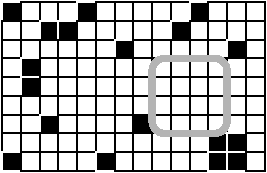
\includegraphics{plus_grand_carre}}
\end{figure}

% \section{Ensemble indépendant de poids maximum dans un arbre}

% Un ensemble $S\subseteq V$ est indépendant dans le graphe $G(V,E)$ si les sommets de $S$ ne sont pas reliés par une arête.
% Étant donné une pondération $w:V\rightarrow \mathbb N$, trouvez un ensemble indépendant $S$ qui maximise $\sum_v\in S w_v$.  C'est un problème NP-difficile, mais très facile pour les arbres.  Donnez un programme dynamique de complexité linéaire pour ce problème.  Indice: choisissez un sommet arbitraire comme racine pour définir la notion de sous-arbre.

\section{Plus long chemin dans un arbre}

Étant donné un arbre $G(V,E)$ calculez la longueur du plus long chemin dans l'arbre.  Ceci peut être fait par deux parcours en profondeur, mais pour cet exercice donnez un programme dynamique.

\begin{figure}[h]
\centerline{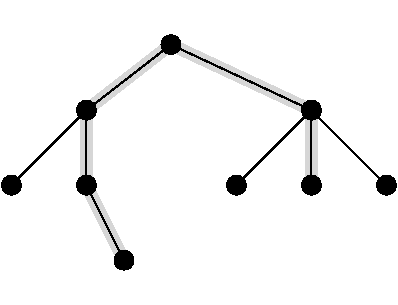
\includegraphics{chemin_arbre}}
\end{figure}

\newpage

\section{Jeux avec des pièces alignées}

Vous jouez un jeu avec votre nièce Sigrid.  Sur la table sont alignées des pièces ayant chacune une différente valeur, disons $w_1$ à $w_n$ Euros dans l'ordre de gauche à droite.  À tour de rôle, chacun de vous prend une des deux pièces extrêmes, toute à gauche ou toute à droite.  Sigrid commence. Quand il n'y a plus de pièces sur la table, vous comparez le total des pièces ramassées.  La personne avec la plus grande somme gagne.
\begin{figure}[ht]
\begin{center}
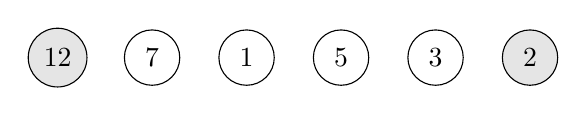
\begin{tikzpicture}[scale=0.3]
\node[circle,draw,minimum size=2em,fill=gray!20] at (0,0)  {12};
\node[circle,draw,minimum size=2em] at (4,0)  {7};
\node[circle,draw,minimum size=2em] at (8,0)  {1};
\node[circle,draw,minimum size=2em] at (12,0)  {5};
\node[circle,draw,minimum size=2em] at (16,0)  {3};
\node[circle,draw,minimum size=2em,fill=gray!20] at (20,0)  {2};
\end{tikzpicture}
\end{center}
% \caption{Une configuration du jeux. Le prochaine joueur peut prendre une des deux pièces grises.}
\end{figure}


\begin{enumerate}
    \item Donnez un programme dynamique pour maximiser votre gain, dans le cas où Sigrid essaye de maximiser son gain à elle.
    \item (Bonus) Montrez pour $n$ pair, vous ne pouvez pas gagner strictement. Indice: ne pensez plus \emph{programmation dynamique} mais \emph{Zugzwang}.
\end{enumerate}


\section{Pavage par des dominos}

Un domino est une forme géométrique qui couvre exactement deux cases sur une grille.  Un pavage d'une grille par des dominos est un placement de dominos qui couvre chaque case exactement une fois, et tel qu'aucun domino ne dépasse la grille.  On cherche à déterminer le nombre de pavages possible d'une grille de 3 lignes et de $n$ colonnes, pour $n$ pair.

\begin{center}
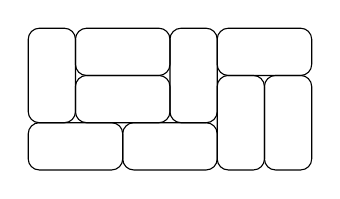
\begin{tikzpicture}[scale=0.6,rounded corners]
\draw (0,0) rectangle (2,1);
\draw (0,1) rectangle (1,3);
\draw (1,1) rectangle (3,2);
\draw (1,2) rectangle (3,3);
\draw (2,0) rectangle (4,1);
\draw (3,1) rectangle (4,3);
\draw (4,0) rectangle (5,2);
\draw (4,2) rectangle (6,3);
\draw (5,0) rectangle (6,2);
\end{tikzpicture}
\end{center}

\begin{enumerate}
    \item Donnez un programme dynamique de complexité $O(n)$  pour ce problème.
    \item Trouvez une autre méthode pour résoudre ce problème en temps $O(\log n)$.
    \item Maintenant si une opération arithmétique ne prend plus un temps constant mais dépend du nombre de bits des nombres concernés, alors quelle est la complexité~?
\end{enumerate}

\source{pour la dernière question: Algorithms, Jeff Erickson, section 5.1.6}
\end{document}